\documentclass{article}[10pt]
\usepackage[pdftex]{graphicx}
\usepackage{amsfonts}
\usepackage[italian]{babel}
%\`
%****************enlarge layout
\textheight     243.5mm
\topmargin      -20.0mm
\textwidth      480pt
\hoffset        -80pt
%*****************theorems and such
\newcounter{esnu}
\newenvironment{esercizio}{\medskip \noindent {\bf Esercizio\addtocounter{esnu}{1} \arabic{esnu}}}{}
\pagestyle{empty}
\newcommand{\liff}{\mathrel{\leftrightarrow}}   % Logical IFF Symbol
\newcommand{\metaiff}{\Longleftrightarrow}      %iff in metatheory

\begin{document}

%\begin{tabular}{llclcr}
% \hspace{-35pt} &{\bf COGNOME:} & \hspace{100pt}        &{\bf NOME:}    & \hspace{100pt}        &{\bf MATRICOLA:}%\hspace{35pt} \\
%\hline
%\end{tabular}
\begin{center} {\bf Esame di Programmazione II, 27 settembre 2013 (2 ore)}\end{center}

Si consideri una gerarchia di classi che rappresentano dei numeri naturali:
%
\begin{center}
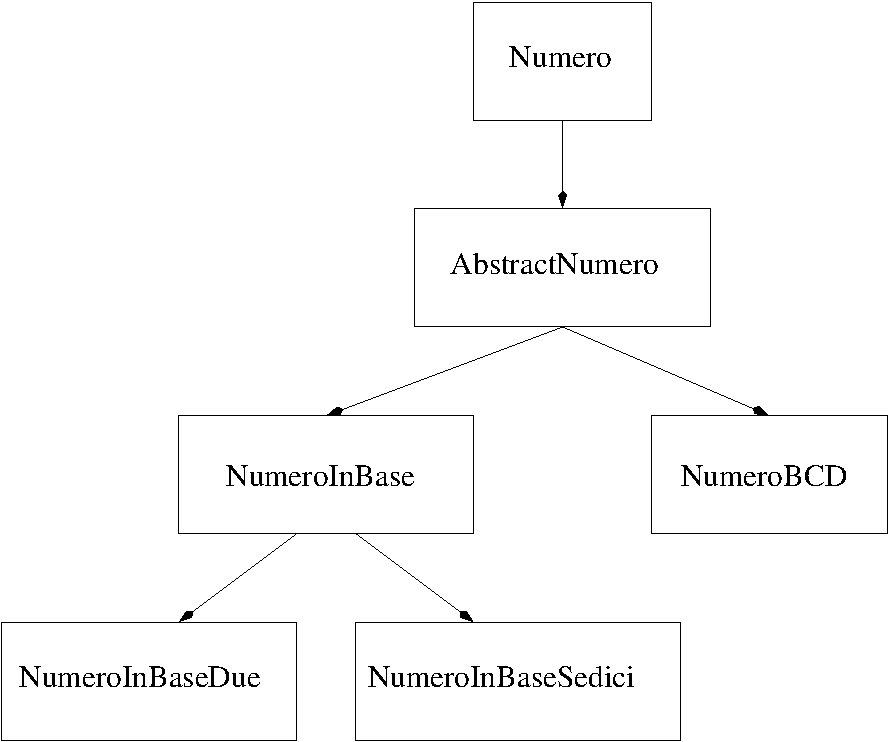
\includegraphics[width=8.5cm]{classi.pdf}
\end{center}

\noindent
L'interfaccia \texttt{Numero} \`e definita come:
%
{\small
\begin{verbatim}
public interface Numero extends Comparable<Numero> {
  public int getValue();
  public void aggiungi(Numero n);
  public void sottrai(Numero n);
}
\end{verbatim}
}

\noindent
dove il metodo \texttt{getValue} restituisce il valore intero del numero e i metodi
\texttt{aggiungi} e \texttt{sottrai} modificano il numero aggiungendo o sottraendone un altro,
rispettivamente. Se la sottrazione desse origine a un numero negativo, dovrebbe venire lanciata un
\texttt{java.lang.ArithmeticException}.
La comparazione fra due numeri \`e il loro ordinamento rispetto al valore crescente.
Due numeri sono uguali se e solo se hanno lo stesso valore.

\begin{esercizio}
\textbf{[5 punti]}
Si scriva la classe astratta \texttt{AbstractNumero} che implementa,
\underline{come \texttt{final}}, i metodi
\texttt{getValue}, \texttt{aggiungi}, \texttt{sottrai}, \texttt{compareTo},
\texttt{equals} e \texttt{hashCode}. Due numeri devono essere considerati
\texttt{equals} se e solo se hanno lo stesso valore.
Se servono campi, devono essere dichiarati \texttt{private}.
Se servono costruttori, devono essere dichiarati \texttt{protected}.
\end{esercizio}

\begin{esercizio}
\textbf{[1 punti]}
Si scriva la classe astratta \texttt{NumeroInBase} che implementa un numero in una base
di numerazione tra due e sedici. Deve fornire un metodo \underline{\texttt{final}}
\texttt{getBase} che restituisce la base di numerazione del numero. Deve avere un costruttore
{\small
\begin{verbatim}
protected NumeroInBase(int value, int base) 
\end{verbatim}
}

\noindent
che costruisce il numero \texttt{value} nella base indicata e che lancia una
\texttt{java.lang.IllegalArgumentException} se il valore \`e negativo
o se la base non \`e fra due e sedici.
\end{esercizio}

\begin{esercizio}
\textbf{[4 punti]}
Si scriva la classe concreta \texttt{NumeroInBaseDue} che
implementa un numero in
base due (la normale codifica binaria dei numeri interi).
Deve avere un costruttore
{\small
\begin{verbatim}
public NumeroInBaseDue(int value)
\end{verbatim}
}

\noindent
che costruisce il numero \texttt{value} in base due e che lancia una
\texttt{java.lang.IllegalArgumentException} se il valore \`e negativo.
Deve avere un metodo \texttt{toString} che restituisce una stringa che descrive
il numero (quindi fatta solo di \texttt{'0'} e \texttt{'1'}).
\end{esercizio}

\begin{esercizio}
\textbf{[4 punti]}
Si scriva la classe concreta \texttt{NumeroInBaseSedici} che implementa un numero in
base sedici (la normale codifica esadecimale dei numeri interi).
Deve avere un costruttore
{\small
\begin{verbatim}
public NumeroInBaseSedici(int value)
\end{verbatim}
}

\noindent
che costruisce il numero \texttt{value} in base sedici e che lancia una
\texttt{java.lang.IllegalArgumentException} se il valore \`e negativo.
Deve avere un metodo \texttt{toString} che restituisce una stringa che descrive
il numero in esadecimale.
\end{esercizio}

\begin{esercizio}
\textbf{[6 punti]}
La rappresentazione \emph{binaria a codice decimale} (bcd) \`e un modo di scrivere in
binario i numeri decimali non negativi, in cui si riservano quattro cifre binarie per ogni cifra
decimale. Per esempio, il numero decimale $209$ viene scritto in bcd come:
\[
  \underbrace{0010}_2\underbrace{0000}_0\underbrace{1001}_9
\]
Si scriva la classe concreta \texttt{NumeroBCD} che implementa un numero in
binario a codice decimale. Deve avere un costruttore
{\small
\begin{verbatim}
public NumeroBCD(int value)
\end{verbatim}
}

\noindent
che costruisce il numero \texttt{value} in binario a codice decimale e che lancia una
\texttt{java.lang.IllegalArgumentException} se il valore \`e negativo.
Deve avere un metodo \texttt{toString} che restituisce una stringa che descrive
il numero in binario a codice decimale (quindi fatta solo di \texttt{'0'} e \texttt{'1'}).
\end{esercizio}

\begin{center}
* * * * *
\end{center}

Se tutto \`e corretto, l'esecuzione del seguente programma:
%
{\small
\begin{verbatim}
import java.util.HashMap;
import java.util.Map;
import java.util.Set;
import java.util.TreeSet;

public class Main {
  public static void main(String[] args) {
    Numero n1 = new NumeroInBaseDue(2034);
    Numero n2 = new NumeroInBaseSedici(2034);
    Numero n3 = new NumeroBCD(2034);
    System.out.println("n1=" + n1);
    System.out.println("n2=" + n2);
    System.out.println("n3=" + n3);
    n2.aggiungi(n3);
    n2.aggiungi(n1);
    n2.sottrai(new NumeroBCD(136));
    System.out.println("n2=" + n2);

    Map<Numero, String> map = new HashMap<Numero, String>();
    map.put(n1, "duemilatrentaquattro in base due");
    map.put(n3, "duemilatrentaquattro in binario a codice decimale");
    System.out.println(map.get(n1)); // cosa stampa?

    // java.util.TreeSet e' un insieme ordinato in senso crescente rispetto a compareTo
    Set<Numero> insieme = new TreeSet<Numero>();
    insieme.add(n1);
    insieme.add(n2);
    insieme.add(n3); 
    System.out.println(insieme); // cosa stampa?
  }
}
\end{verbatim}
}

\noindent
deve stampare:
%
{\small
\begin{verbatim}
n1=11111110010
n2=7f2
n3=0010000000110100
n2=174e
........................
........................
\end{verbatim}
}

\begin{esercizio}
\textbf{[2 punti]}
Cosa viene stampato (al posto dei puntini) dalle ultime due istruzioni
\texttt{System.out.println} del metodo \texttt{main} della classe \texttt{Main}?
Perch\'e?
\end{esercizio}

\end{document}
